\documentclass[tikz,border=10pt]{standalone}
\usetikzlibrary{positioning}
\begin{document}
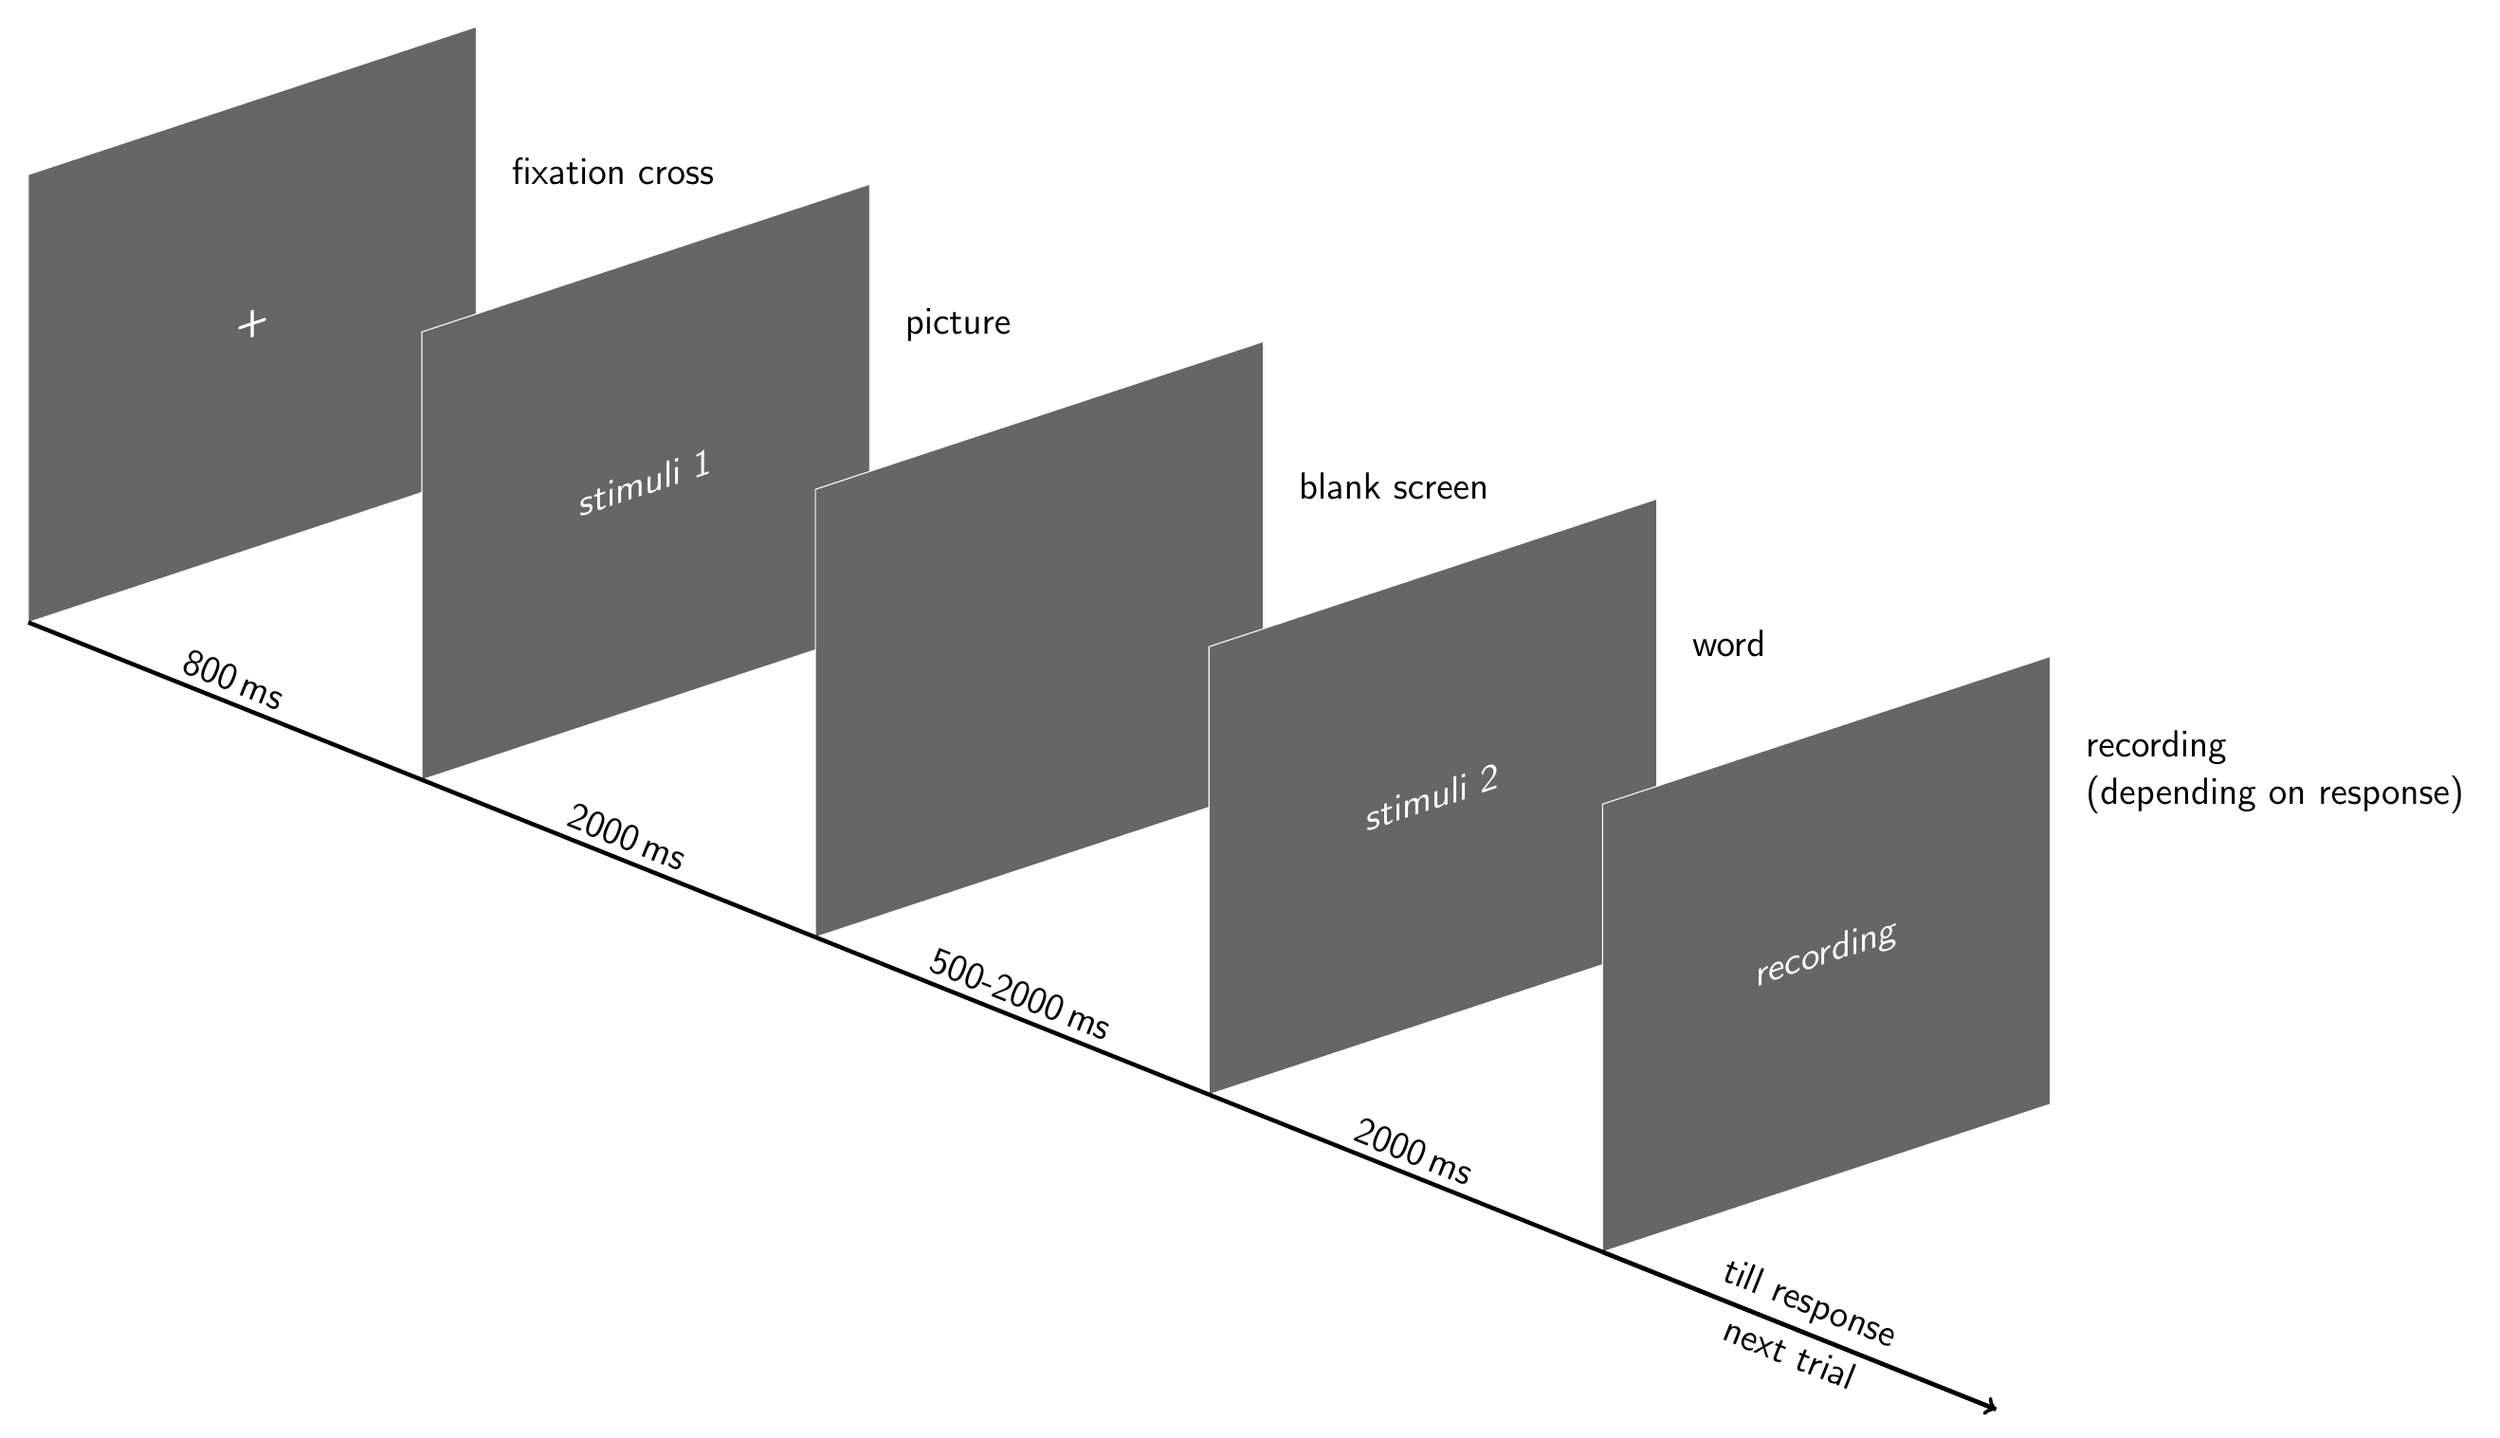
\begin{tikzpicture}
	\tikzset{
		basefont/.style = {font = \Large\sffamily},
		timing/.style = {basefont, sloped,above,},
		label/.style = {basefont, align = left},
		screen/.style = {basefont, white, align = center,
				minimum size = 6cm, fill = black!60, draw = white}};

	% macro for defining screens
	\newcommand*{\screen}[4]{%
		\begin{scope}[xshift  =#3, yshift = #4,
				every node/.append style = {yslant = 0.33},
				yslant = 0.33,
				local bounding box = #1]
			\node[screen] at (3cm,3cm) {#2};
		\end{scope}
	}
	% define several screens
	\screen{frame1}{\textbf+} {0}     {0}
	\screen{frame2}{stimuli 1}{150} {-60}
	\screen{frame3}{}         {300}{-120}
	\screen{frame4}{stimuli 2}{450}{-180}
	\screen{frame5}{recording}{600}{-240}
	\coordinate [xshift=750,yshift=-300] (frame6);

	% add annotations
	\foreach \i / \content in {
			1/fixation cross,
			2/picture,
			3/blank screen,
			4/word,
			5/recording\\(depending on response)
		}
	\node[label, above right=5em and 1em of frame\i.east]
	(f\i-label) {\content};

	% add time course
	\foreach \j [count=\i] / \content in {
			2/800\,ms,
			3/2000\,ms,
			4/500-2000\,ms,
			5/2000\,ms,
			6/till response
		}
	\path[ultra thick] (frame\i.south west) edge
	node[timing] {\content} (frame\j.south west);

	% some manual addition
	\path[ultra thick,->] (frame5.south west) edge
	node[timing, below] {next trial} (frame6);
\end{tikzpicture}
\end{document}
